\apendice{Descripción de adquisición y tratamiento de datos}


\section{Descripción formal de los datos}

En este trabajo, se han empleado imágenes de radiografía de tórax (CXT por sus siglas en inglés), en un formato \textit{.jpeg} obtenidas a partir de una base de datos pública ~\cite{kaggle24}. En esta base de datos, se encuentra una carpeta principal con diversas subcarpetas donde se alojan las imágenes.

La carpeta principal contiene 3 subcarpetas, la de entrenamiento (\textit{train}), validación (val) y prueba (test). Dentro de cada una de estas carpetas hay dos subcarpetas, ``NORMAL'', con las imágenes sin neumonía y ``PNEUMONIA'' con las imágenes de CXT que presentan neumonía.

A su vez, las carpetas de ``PNEUMONIA'' tienen indicado en el nombre del archivo (la imagen) si se trata de una neumonía viral o bacteriana. 

\begin{itemize}
    \item Las imágenes de entrenamiento o \textit{train} se emplean para entrenar el modelo de aprendizaje automático ~\cite{linkdif24}. Dentro de la carpeta ``\textit{train}'', ``NORMAL'' hay un total de 1341 imágenes, y en ``\textit{train}'', ``PNEUMONIA'' hay 3875 imágenes.
    \item Las imágenes de prueba o \textit{test} se emplean para evaluar el rendimiento del modelo después del proceso de entrenamiento y validación. Proporciona una escena objetiva de la precisión del modelo para generalizar datos nuevos ~\cite{linkdif24}. Dentro de la carpeta ``\textit{test}'', ``NORMAL'' hay un total de 234 imágenes, y en ``\textit{test}'', ``PNEUMONIA'' hay 390 imágenes.
    \item Las imágenes de validación o val son una carpeta adicional que ayuda a seleccionar el mejor modelo y evitar el sobreajuste ~\cite{linkdif24}. Dentro de la carpeta ``val'', ``NORMAL'' hay un total de 8 imágenes, y en ``val'', ``PNEUMONIA'' hay 8 imágenes.
\end{itemize}

Las imágenes estaban distribuidas de manera desigual en las carpetas de entrenamiento (\textit{train}) y validación (val). La carpeta de validación contenía únicamente 16 imágenes, mientras que, la carpeta de entrenamiento contenía 5216 imágenes. Esta distribución desbalanceada puede afectar negativamente a la calidad del entrenamiento y la validación del modelo de IA, ya que, una muestra de validación tan pequeña no es representativa y no proporciona una evaluación precisa del rendimiento del modelo. De forma que, se ha creado una nueva distribución de las imágenes.
En la nueva distribución, un 64\% de las imágenes han sido destinadas a \textit{train}, un 20\% para \textit{test} y un 16\% para val. De la misma manera, las imágenes han sido redistribuidas de manera proporcional en cada una de las subcarpetas ``NORMAL'' y ``PNEUMONIA''.

Cada imagen posee un valor distinto de pixeles, es por ello que, antes de comenzar a trabajar con ellas, se realiza un preprocesamiento de imágenes para asociarles a todas ellas el mismo número de pixeles. En este preprocesamiento, también se realiza una normalización de los datos al reescalar los pixeles, de forma que pasan de estar entre un valor de 1 y 255 a estar entre los valores 0 y 1 para poder trabajar correctamente con ellas.

    
\section{Descripción clínica de los datos.}

\subsection{Cosas a tener en cuenta para la realización de una radiografía de rayos X}

Antes meterse en profundidad con las imágenes de radiografía de tórax (CXT por sus siglas en inglés), se van a mencionar algunos puntos importantes a tener en cuenta antes y durante la realización de una radiografía de rayos X:
\begin{itemize}
    \item Se debe verificar la identidad del paciente antes de la realización de la prueba ~\cite{gelaw15}.
    \item El objetivo principal es obtener imágenes de buena calidad a la primera para minimizar la exposición a los rayos X, aunque, si esto no es así, deberán ser desechadas y repetir el proceso ~\cite{gelaw15}.
    \item El paciente debe ser informado acerca de la posición que debe tener su cuerpo y la respiración (inspiración y expiración) que debe realizar ~\cite{gelaw15}.
    \item Se tiene que dar al paciente la bata para ponerse y se deben evitar objetos metálicos alrededor del pecho y cuello (pendientes, collares, etc.) ~\cite{gelaw15}.
    \item Los pacientes con discapacidad tienen preferencia y, en el caso de pacientes con problemas de audición, la explicación tiene que realizarse de forma simbólica o con ayuda del acompañante ~\cite{gelaw15}.
    \item En ocasiones, puede ser necesaria la realización de radiografías desde otras vistas (lateral, oblicua, etc.) para una mejor visualización ~\cite{gelaw15}.
    \item Se debe proteger tanto al personal como al paciente y los acompañantes de la exposición a rayos X. Por ello, se deben aplicar ciertas medidas: emplear una radiación lo más baja posible, proporcionar un delantal de plomo a todos los solicitantes con una protección extra para mujeres embarazadas, las puertas de rayos X deben estar cerrades durante la exposición a la radiación, el personal debe permanecer en una sala protegida durante la exposición y se les debe realizar mediciones periódicas para controlar la radiación, se debe asegurar que la radiación no salga de las salas de rayos X y, por último, las salas de rayos X deben tener una señal de advertencia ~\cite{gelaw15}. 
    
\end{itemize}

Aunque la vista principal para la realización de una CXT es la proyección postero anterior (PA), donde el paciente se sitúa frente a la placa de imagen, en ocasiones con esta vista no se ve claramente alguna anomalía, por lo que, para confirmar o excluir la sospecha, es necesaria la realización de imágenes desde otras vistas ~\cite{gelaw15}:
\begin{itemize}
    \item \textbf{Vista/posición lateral}: se sitúa el lado de interés cerca del detector durante la exposición de la radiación. La imagen se etiqueta según el lado que se coloque frente al detector, por ejemplo, si es el lado derecho, la imagen quedaría etiquetada como ``lateral derecho'' ~\cite{gelaw15}. Figura \ref{fig:CXR_vista_lateral}.
    
    \begin{figure}[!h]
        \centering
        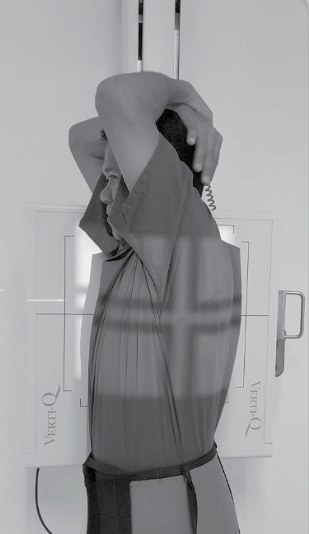
\includegraphics[width=0.30\textwidth]{img/CXR_vista_lateral.PNG}
        \caption{CXT vista lateral. ~\cite{gelaw15}.}
        \label{fig:CXR_vista_lateral}
    \end{figure}
    \FloatBarrier

    \item \textbf{Proyección lordótica}: la parte posterior superior del tórax se sitúa en contacto con el detector. Con esta prueba se consigue que las costillas se alineen longitudinalmente con el haz de rayos X y las clavículas se levanten por encima de los pulmones para poder obtener una vista sin obstáculos de los ápices pulmonares (parte superior del pulmón) y una visualización clara entre las costillas siempre que la técnica y la anatomía lo permitan ~\cite{gelaw15}. Figura \ref{fig:cxr_lordotica}.
    
    Esta vista tiene una variante en la cual el paciente en lugar de tener la parte posterior superior del tórax en contacto con el detector, la parte que tiene en contacto con el detector es la parte anterior inferior del tórax. Es especialmente útil para visualizar los lóbulos inferiores del pulmón desde un ángulo distinto ~\cite{gelaw15}.

    \begin{figure}[h]
        \centering
        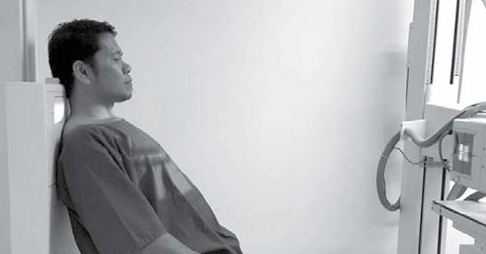
\includegraphics[width=0.55\textwidth]{img/cxr_lordotica.PNG}
        \caption{CXT proyección lordótica. ~\cite{gelaw15}.}
        \label{fig:cxr_lordotica}
    \end{figure}
    \FloatBarrier

    \item \textbf{Posición en decúbito lateral}: el paciente se encuentra tumbado de un lado o del otro y permite determinar la presencia de líquido pleural y neumotórax. Al igual que ocurre con la vista lateral, la imagen se etiqueta según el lado que se coloque frente al detector ~\cite{gelaw15}. Figura \ref{fig:cxr_decubito_lateral}.

    \begin{figure}[h]
        \centering
        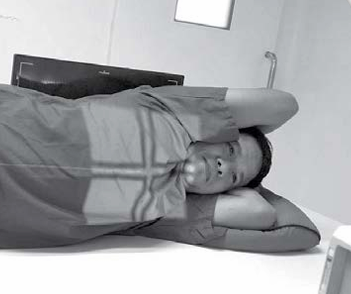
\includegraphics[width=0.50\textwidth]{img/cxr_decubito_lateral.PNG}
        \caption{CXT decúbito lateral. ~\cite{gelaw15}.}
        \label{fig:cxr_decubito_lateral}
    \end{figure}
    \FloatBarrier

    \item \textbf{Vista oblicua}: existen cuatro tipos distintos: oblicua anterior derecha, anterior izquierda, posterior derecha y posterior izquierda. Se puede realizar en posición vertical o tumbado (en caso de que el paciente no pueda mantenerse de pie). Las proyecciones oblicuas anteriores se emplean para la visualización de los pulmones y el mediastino y las vistas oblicuas posteriores se emplean generalmente para la visualización de las costillas y la caja torácica, aunque también pueden realizarse para ver áreas de los pulmones ~\cite{gelaw15}. Se realiza poniendo una de las manos sobre la cabeza tal y como se muestra en la figura \ref{fig:cxr_posterior_oblicua}.

    \begin{figure}[h]
        \centering
        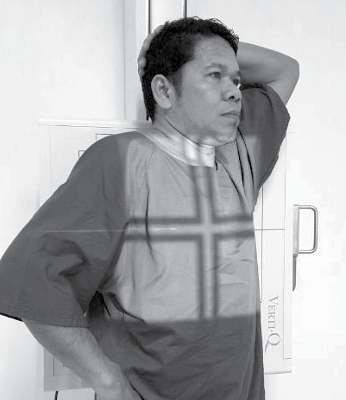
\includegraphics[width=0.40\textwidth]{img/cxr_posterior_oblicua.PNG}
        \caption{CXT posterior oblicua. ~\cite{gelaw15}.}
        \label{fig:cxr_posterior_oblicua}
    \end{figure}
    \FloatBarrier

    \item \textbf{Vista anteroposterior}: se trata de una alternativa a la CXT en posición PA. El paciente se encuentra tumbado con la cara anterior del tórax mirando hacia el detector. Tiene especial interés en personas mayores que no puedes mantenerse de pie o pacientes pediátricos en la misma situación ~\cite{gelaw15}. Por lo tanto, esta CXT puede ser de gran relevancia para este proyecto ya que se trabaja con pacientes de entre 1 y 5 años. Figura \ref{fig:cxr_anteoposterior}.

    \begin{figure}[h]
        \centering
        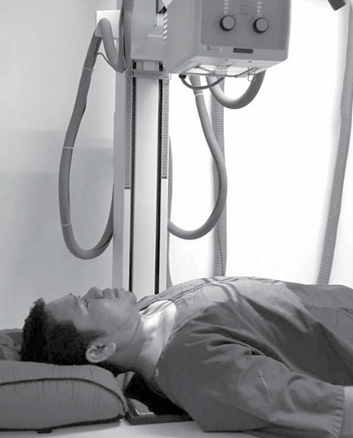
\includegraphics[width=0.40\textwidth]{img/cxr_anteoposterior.PNG}
        \caption{CXT anteoposterior. ~\cite{gelaw15}.}
        \label{fig:cxr_anteoposterior}
    \end{figure}
    \FloatBarrier

    
\end{itemize}

Las radiografías de tórax proporcionan imágenes en blanco y negro donde los huesos se observan de color blanco debido a que bloquean la radiación mientras que los pulmones (al estar llenos de aire) o el aire en sí aparecen como zonas más negras. El corazón también se observa como una zona clara ~\cite{Mayoclinic24}.

Además de contener la imagen correspondiente, las radiografías de tórax también incluyen información biológica relacionada con el paciente para asegurarse que, la imagen pertenece a ese paciente y analizarla correctamente acorde a su edad, sexo, etc. El radiólogo también debe asegurarse de la correcta calidad de la imagen ~\cite{gelaw15}.

\subsection{Análisis de imágenes de CXT}

A la hora de analizar el médico especializado la CXT, lo hace de manera sistemática, es decir, observa de forma ordenada todas las partes de la imagen para detectar posibles anomalías. Una forma de visualizar estas imágenes es comenzar observando las costillas que recubren los pulmones, la columna vertebral, los diafragmas y los recesos costodiafragmáticos. Después, se pasa al corazón y el mediastino y, finalmente a los pulmones. A la hora de ver los pulmones, también se analiza región a región. Este proceso se realiza hasta que todas las zonas de la imágen hayan sido analizadas correctamente ~\cite{gelaw15}.

\begin{itemize}
    \item \textbf{Corazón}: órgano principal del sistema circulatorio que se encarga de bombear sangre a diversos tejidos del cuerpo. Se encuentra en la cavidad torácica, por detrás del esternón y las costillas. El lado derecho del corazón recibe sangre venosa del organismo, es decir, con dióxido de carbono, mientras que, el lado izquierdo del corazón recibe sangre arterial, es decir, sangre oxigenada. Late con una frecuencia de entre 40 y 60 latidos por minuto y tiene un tamaño similar al de un puño ~\cite{CliUniNaCorazon24, CliUniNaSaVenosa24}.
    \item \textbf{Pulmones}: par de órganos ubicados en la cavidad torácica encargados de la función respiratoria y del intercambio de gases entre el aire y la sangre ~\cite{CliUniNaPulmon24}.
    \item \textbf{Costillas}: están constituidas por doce pares de huesos planos, largos y curvos que forma la caja torácica ~\cite{CliUniNaCostilla24}. Su principal función consiste en proteger a los órganos torácicos internos ~\cite{kenhub24}. Otras de sus funciones es la de estructura pasiva en el proceso de la respiración ~\cite{CliUniNaCostilla24}.

    Las costillas se pueden dividir en verdaderas y falsas. Las verdaderas son aquellas que están conectadas directamente con el esternón mientras que las falsas, se conectan al esternón por medio de un cartílago común. Las dos últimas costillas son las también denominadas costillas flotantes ya que, no llegan al esternón ~\cite{CliUniNaCostilla24, kenhub24}. 
    \item \textbf{Columna vertebral}: conjunto de huesos, tendones, músculos y otros tejidos que se extienden desde el cráneo hasta el coxis. Su función consiste en proteger la médula espinal y dar soporte al tronco ~\cite{NIHColVer24, MedliColVer24}
    \item \textbf{Diafragmas}: músculo delgado en forma de cúpula que separa el tórax del abdomen. Se encuentra debajo del corazón y los pulmones. Interviene en el proceso de la respiración ya que, al inhalar se contrae permitiendo que los pulmones se llenen de aire y, al exhalar se relaja permitiendo salir el aire de los pulmones ~\cite{NIHDiaf24, MedliColDiaf24, premiummadridDiaf24}.
    \item \textbf{Recesos costodiafragmáticos}: se trata del espacio entre la pared costal y el diafragma. Interviene en el proceso de la respiración ya que, permite que el diafragma se mueva eficientemente. La presencia de aire, líquido o algún tejido puede indicar la existencia de patologías como cáncer, neumotórax o efusiones pleurales por lo que, es de gran ayuda en el diagnóstico de enfermedades pulmonares ~\cite{CliUniNaReCostodiaf24}.
    \item \textbf{Mediastino}: área anatómica entre los pulmones que engloba órganos como el corazón, los vasos sanguíneos grandes, la tráquea, el timo, el esófago, los bronquios y los ganglios linfáticos ~\cite{NIHmediastino24}.
    
\end{itemize}

Además, en una CXT también se examinan cuidadosamente otras áreas ocultas como las clavículas, vías biliares, ganglios paratraqueales y espacio retrocardiaco ~\cite{gelaw15}.

\begin{itemize}
    \item \textbf{Clavícula}: cada uno de los dos huesos alargados situados en la parte superior del pecho. 
    
    Se articula por su extremo distal con la escápula y por el proximal con el esternón ~\cite{CliUniNaClavicula24, RealAcaEsClavicula24}.
    \item \textbf{Vías biliares}: conductos que conectan el hígado, el intestino delgado y la vesícula biliar de forma que, transportan la bilis desde el hígado hasta el intestino delgado ~\cite{CliUniNabilis24}. 
    
    La bilis es una sustancia generada por el hígado y almacenada en la vesícula biliar. Desempeña un papel importante en la digestión, absorción de las grasas y eliminación de deshechos ~\cite{CliUniNabilis24}.
    \item \textbf{Ganglios paratraqueales}: nodos linfáticos ubicados en la tráquea. Su principal función consiste en combatir las infecciones capturando virus, bacterias y otros agentes patógenos ~\cite{MaCliGanLin24, imaiosGanLin24}.
    \item \textbf{Espacio retrocardiaco}: se trata de un espacio ubicado en el mediastino que queda oculto por el corazón en una CXT frontal permitiendo ver una patología en esa zona cuando aumenta su densidad. Por lo tanto, se convierte en un espacio fundamental para identificar en una radiografía lateral de tórax una posible anomalía en la zona del mediastino ~\cite{canals2022espacio}.
\end{itemize}

A la hora de analizar una imagen de CXT con anomalías evidentes, es importante no dejar pasar otras anomalías más sutiles ~\cite{gelaw15}.

Las anomalías tienen que describirse de la forma más completa posible, esto incluye tipo, ubicación, tamaño, densidad u homogeneidad entre otras ~\cite{gelaw15}.

En imágenes de CXT con una anomalía se pueden distinguir tres tipos: 

\begin{enumerate}
    \item Cambio en la apariencia de la estructura
    \item Área anormalmente blanca (cuando debería ser oscura)
    \item Área anormalmente oscura (cuando debería ser blanca)
\end{enumerate}

En el caso concreto de la neumonía, estaríamos hablando del segundo tipo de anomalía ``área anormalmente blanca'' ya que, los pulmones al absorber poca radiación deberían verse de color oscuro pero, al existir neumonía, se aprecian opacidades blancas en el pulmón denominadas infiltrados pulmonares ~\cite{gelaw15}. 

Los \textbf{infiltrados pulmonares} son alteraciones en los pulmones que se observan como opacidades mal definidas en imágenes como radiografías de tórax. Estas opacidades son cambios en el tejido pulmonar que indican una enfermedad o secuela de una enfermedad pulmonar. Sus causas pueden ser infecciosas, oncológicas, etc  ~\cite{Doctoralia24}. Los infiltrados pulmonares u opacidades blancas se encuentran perfectamente explicados en el apartado de ``Conceptos teóricos'' de la memoria.



